\section{Quantum Circuits}
For this research we have chosen to execute the Teleportation protocol, Grover's search algorithm, Entanglement Swapping and Entanglement Purification on the devices. The circuits are all made using an open source software development kit called Qiskit, which uses Python as its main programming language. The written codes, made with Jupyter Notebook, for the circuits can be found in appendix {\color{red} \emph{number}}. In the following we will describe the circuits, mainly focussing on ... and {\color{red}\emph{the measurement of the circuits}}. Thereafter, the measurement protocols will be described.

\subsection{The Teleportation protocol}
\label{sub:tele}
Quantum teleportation is a procedure where a quantum state can be transmitted from one location to the other. Usually this is done by creating an arbitrary state $\ket{\psi}$ on the first qubit and a $\ket{\Phi^+}$ Bell-state on the second and third qubit, as can be seen in figure \ref{fig:telgen}.
\begin{figure}[h]
	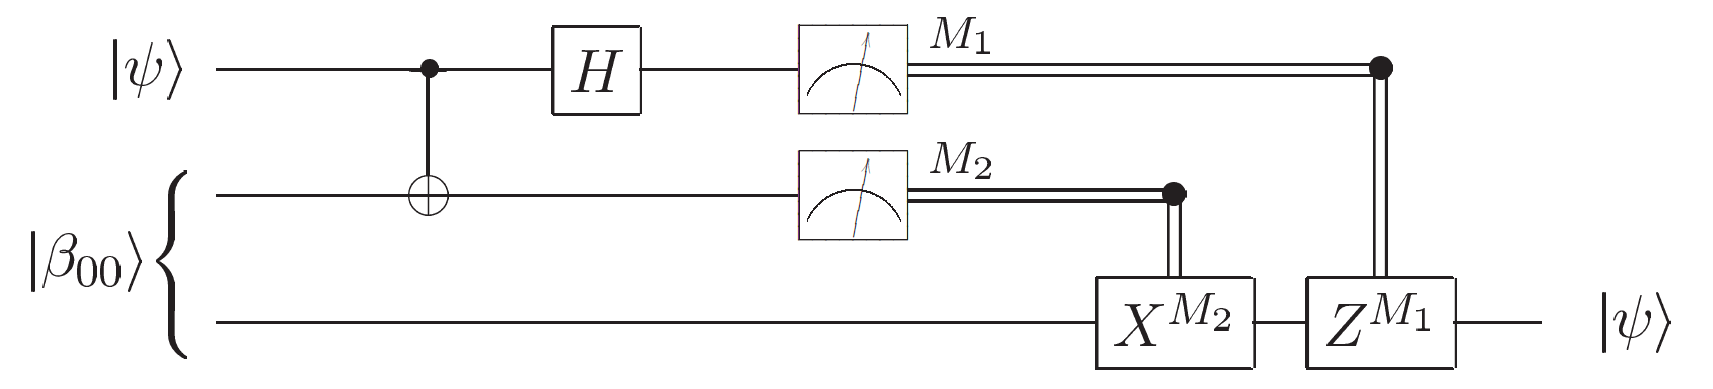
\includegraphics[width=0.48\textwidth]{images/Teleport_general.png}
	\caption{General teleportation protocol circuit. Here the $\ket{\Phi^+}$ Bell-state is denoted as $\ket{\beta_{00}}$.  \cite{nielsen10_quant}}
	\label{fig:telgen}
\end{figure}
Subsequently, a CNOT gate is applied to the second qubit and a Hadamard gate to the first qubit. Now the first and second qubit will be measured in the Z-basis, with the measurement results being $M_1$ and $M_2$, respectively. A X- and/or Z-gate is applied to the third qubit depending on the measurement outcome. If $M_1 = +1$ a Z-gate will be applied and if $M_2 = +1$ a X-gate will be applied. This will result in the state $\ket{\psi}$ being teleported to the third qubit.

However, to know if the state $\ket{\psi}$ is properly transported, the third qubit must be measured. Unfortunately, it is not possible (yet) to apply a gate after a measurement on the used devices. So, we will have to resort to post measurement techniques, as the gates cannot be applied to the third qubit. The circuit that is send to the devices is presented in figure \ref{fig:telcir}.
\begin{figure}[h]
	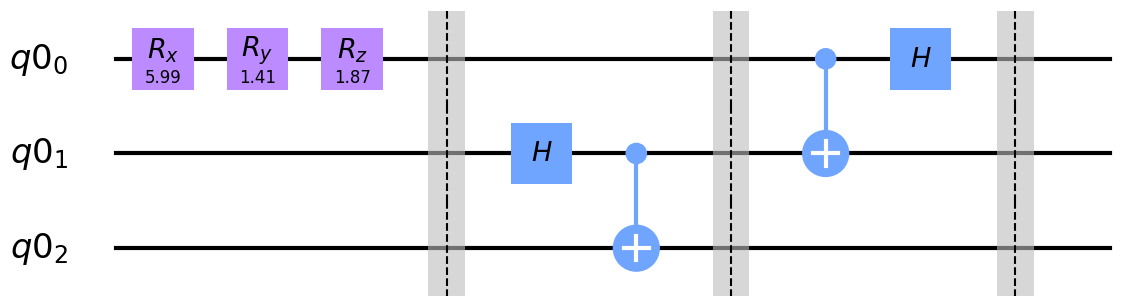
\includegraphics[width=0.48\textwidth]{images/teleport_circuit.png}
	\caption{Teleport circuit used for the measurements. (The operators on the first qubit were randomized every run.)}
	\label{fig:telcir}
\end{figure}
As one can easily see the gates on the third qubit are absent. To account for this, a Pauli-X or Pauli-Z matrix is applied to the final state on the third qubit, after the measurement. Which works similar to the general protocol: if $M_1 = +1$ a Pauli-Z matrix will be applied and if $M_2 = +1$ a Pauli-X matrix will be applied. This will, in post measurement, result in the state $\ket{\psi}$ being teleported to the third qubit.

\subsection{Grover's search algorithm}
The Grover search algorithm can find an input given to a black box with a high likeliness. In our case, the input that is given is a unitary 4x4 diagonal matrix, with three values being +1 and one being -1. The algorithm can find which one of the numbers on the diagonal is -1. The circuit that is used in the measurements is presented in figure \ref{fig:grocir}.
\begin{figure}[h]
	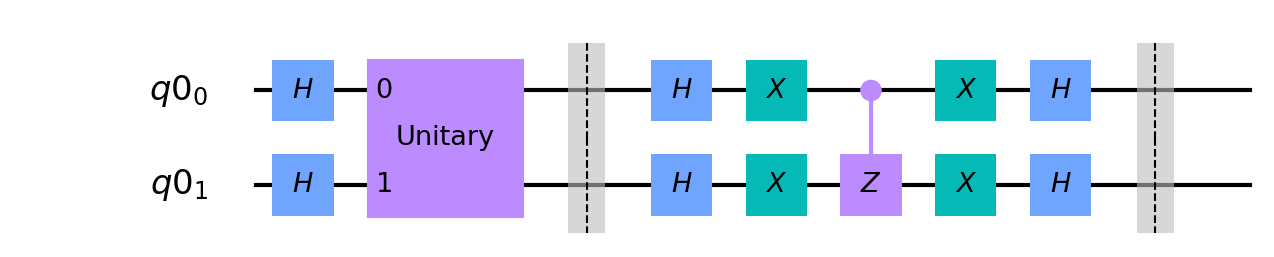
\includegraphics[width=0.48\textwidth]{images/grover_circuit.png}
	\caption{Grover's search algorithm circuit used for the measurements. (The position of the -1 value is randomized every run.)}
	\label{fig:grocir}
\end{figure}
For explanatory reasons, let us choose the unitary matrix to be:
\begin{equation*}
U = 
\begin{bmatrix}
1 & 0 & 0 & 0 \\
0 & 1 & 0 & 0 \\
0 & 0 & 1 & 0 \\
0 & 0 & 0 & -1 
\end{bmatrix}
\end{equation*} 
$U$ is randomized for every run of the circuit on a device or simulator. The two qubit will both start in the $\ket{0}$ state. After the application of the Hadamard gates the total state will be: $\ket{\Psi} = \frac{1}{2}\left(\ket{00}+\ket{01}+\ket{10}+\ket{11}\right)$. Now $U$ is applied giving: $\ket{\Psi} = \frac{1}{2}\left(\ket{00}+\ket{01}+\ket{10}-\ket{11}\right)$.
The part after the unitary in figure \ref{fig:grocir} is important for the Grover's search algorithm and does an inversion about the mean. This inverts the constants multiplied with each state around the mean of the total. In this case the mean is $\frac{3\cdot\frac{1}{2}-\frac{1}{2}}{4} = \frac{1}{4}$. Inverting $\frac{1}{2}$ about the mean, means that it will become 0. For $-\frac{1}{2}$ it will become 1, thus making $\ket{11}$ the only state left. Measuring this will result in $M_1 = M_2 = +1$. This result is related to where in $U$ the -1 value is positioned and in this case the result shows it is in the bottom right corner (where we positioned -1 in the first place).

\subsection{Entanglement swap}
This protocol is, as the name states, a way of changing the entanglement between two qubits, for example the first and second, to an entanglement between different qubits, for example the first and fourth. This circuit will first be generally described, and can be found in figure \ref{fig:swapgen}.
\begin{figure}[h]
	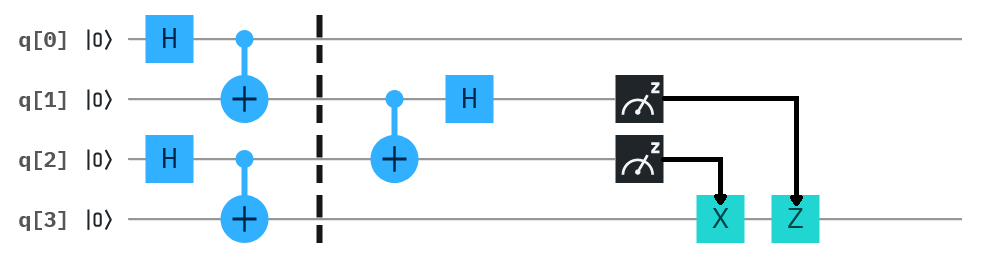
\includegraphics[width=0.48\textwidth]{images/swap_general.png}
	\caption{General entanglement swap protocol circuit. Made using the IBM Quantum experience Circuit Composer.}
	\label{fig:swapgen}
\end{figure}
First, an arbitrary Bell-like state is created on the first two qubits (q[0] and q[1]). For explanatory reasons, this is now a simple $\ket{\Phi^+}$ Bell state. On the third and fourth qubit, a $\ket{\Phi^+}$ state is also created. This gives the following state: $\ket{\Psi} = \frac{1}{2}\left(\ket{0000}+\ket{0011}+\ket{1100}+\ket{1111}\right)$. So at this point our arbitrary state has entanglement with the first and second qubit, which are the fourth and third number in de bra-ket notation, respectively. Now, a CNOT gate is applied between the second and third qubit resulting in: $\ket{\Psi} = \frac{1}{2}\left(\ket{0000}+\ket{0111}+\ket{1100}+\ket{1011}\right)$. After the application of the Hadamard gate to the second qubit we get eight different possible states: 
%Did something weird with the equation here or else it wouldn't fit in the text
$\ket{\Psi} = \frac{1}{\sqrt{8}}(\ket{0000}+\ket{0010}+\ket{0101}-\ket{0111}+\ket{1001}$$-\ket{1011}+\ket{1100}+\ket{1110})$. Now for the measurement part. If the result would be $M_1 = -1$ and $M_2 = +1$, a X-gate is applied to the fourth qubit. This would result in: $\ket{\Psi} = \frac{1}{\sqrt{2}}\left(\ket{0100}+\ket{1101}\right)$. One can see that the first and fourth qubit now have the combined state $\frac{1}{\sqrt{2}}\left(\ket{00}+\ket{11}\right) = \ket{\Phi^+}$, so the entanglement is swapped from the first and the second to the first and the fourth qubit.

However, we have to resort to post measurement techniques. Already stated in the section \ref{sub:tele}.\nameref{sub:tele}, gates cannot be applied after measurement. The circuit that is given to the devices and simulators is shown in figure \ref{fig:swapcir}.
\begin{figure}[h]
	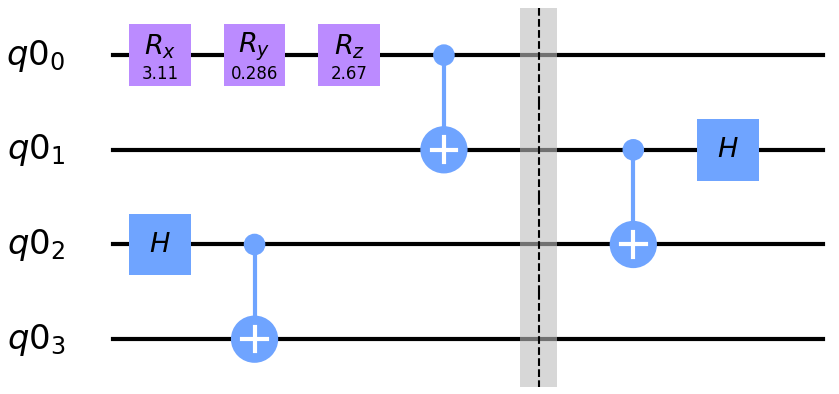
\includegraphics[width=0.48\textwidth]{images/swap_circuit.png}
	\caption{Entanglement swap circuit used in the measurements. Every measurement a random Bell-like state is created on the first two qubits.}
	\label{fig:swapcir}
\end{figure}
At the beginning of every measurement, a random Bell-like state is created. Now, the circuit runs identical to what is explained before, till the measurements take place. After the measurement, a Pauli-X or Pauli-Z matrix is applied to the fourth qubit. This depends on the measurement outcome of $M_1$ and $M_2$. If $M_1 = +1$ we apply a Pauli-Z matrix and if $M_2 = +1$ we apply a Pauli-X matrix. This will give, excluding any errors, an entangled state (post measurement) which we can use for our calculations and comparisons.

\subsection{Entanglement purification}
\emph{Can I have some hype in the chat please?}

F

F

F

F

F

F

F

F

F

F